\chapter{Methode}
Om het project kwalitatief goed uit te kunnen voeren is er gebruik gemaakt van verschillende methoden en technieken. Er is gezien de HBO vaardigheden competenties en kenmerken van het project gekozen voor een agile iteratieve projectmethodiek. Als projectmethodiek is er gekozen voor Kanban, die verder beschreven is in het plan van aanpak \cite{pva}.\par
De reden voor deze aanpak is omdat hiermee werk gestructureerd opgesplitst, ingeschat, geprioriteerd en ingepland wordt in iteraties. Dit geeft de vereiste flexibiliteit om snel te kunnen schakelen bij aanpassingen of nieuwe requirements. Dit vereist het gebruik van experimentele software, materie en technologieën die nog niet bekend waren voordat dit project begon.\par
Deze praktische aanpak maakt het mogelijk dat bevindingen tijdens het onderzoeken naar een onderwerp gelijk gebruikt kunnen worden in een stuk ontwikkeling van het prototype (proof of concept). Verder is er voor Kanban gekozen omdat het project niet in teamverband wordt uitgevoerd. Kanban, in tegenstelling tot Scrum, vereist niet de teamvergaderingen die normaal gesproken nodig zijn als het project in teamverband wordt uitgevoerd (daily standups, retrospectives etc..).\par
Met de uitvoering van Kanban is er gekozen om gebruik te maken van het whiteboard op kantoor, zie figuur \ref{fig:kanbanbord}. Het bord bestaat uit vier kolommen: To Do, In Progress, Review en Done. Net als de bekende Scrum methodiek staat hier al het opgesplitste werk op, voor zowel de school als voor het stagebedrijf. Zo wordt alles eerst onder het kopje To Do gezet. Het werk wat een hoge prioriteit heeft, wordt bovenaan geplaatst. Wanneer ik begin met een nieuwe ticket dan wordt deze verplaatst naar de In Progress kolom. Op het moment dat ik het werk heb afgerond wordt deze eerst opgestuurd voor feedback en acceptatie. Dit gebeurt door de ticket in de review kolom te plaatsen.\par
\newpage

Zodra een ticket goedgekeurd is door de stakeholder, dan wordt het werk als klaar beschouwd. In het geval van het proof of concept onderzoek of analyse documenten, wordt deze review uitgevoerd door de productowner (Daniël Siahaya) of in sommige gevallen door de opdrachtgever (Allianz Group, Arjan Zaal). Het werk voor school wordt vanuit de review kolom naar To Do gezet nadat er feedback ontvangen is van de stagebegeleider en assessor.\par
Door deze aanpak is er één oogopslag duidelijk wat de huidige stand van zaken is. Dit geeft ook inzicht in het proces, want hierdoor wordt al snel duidelijk tegen het einde van een iteratie of er niet te veel nog staat bij de To Do of Doing kolom.\par
Hierdoor kan ik iedere iteratie nieuwe doelstellingen maken en controleren of het project nog op schema ligt. Op momenten dat dit niet zo is, kan er een juiste afstemming gemaakt worden. Deze retrospective \footnote{ https://www.atlassian.com/team-playbook/plays/retrospective} wordt uitgevoerd na iedere iteratie met de bedrijfsbegeleider, waar ik reflecteer op mijn eigen werkprocessen van die iteratie. Deze retrospective momenten hebben in het begin wat meer tijd gekost, maar met het verloop van het project zijn deze momenten steeds minder nodig. Na een iteratie wordt dan ook de resultaten of bevindingen van onderzoek behandeld en gekeken naar wat er te doen staat in de volgende iteratie. Om deze feedback loop zo kort mogelijk te houden is er gekozen voor 2 weken iteraties, zodat er voldoende tijd is om resultaten te boeken en voldoende feedback momenten zijn.
\begin{figure}[h]
    \begin{center}
        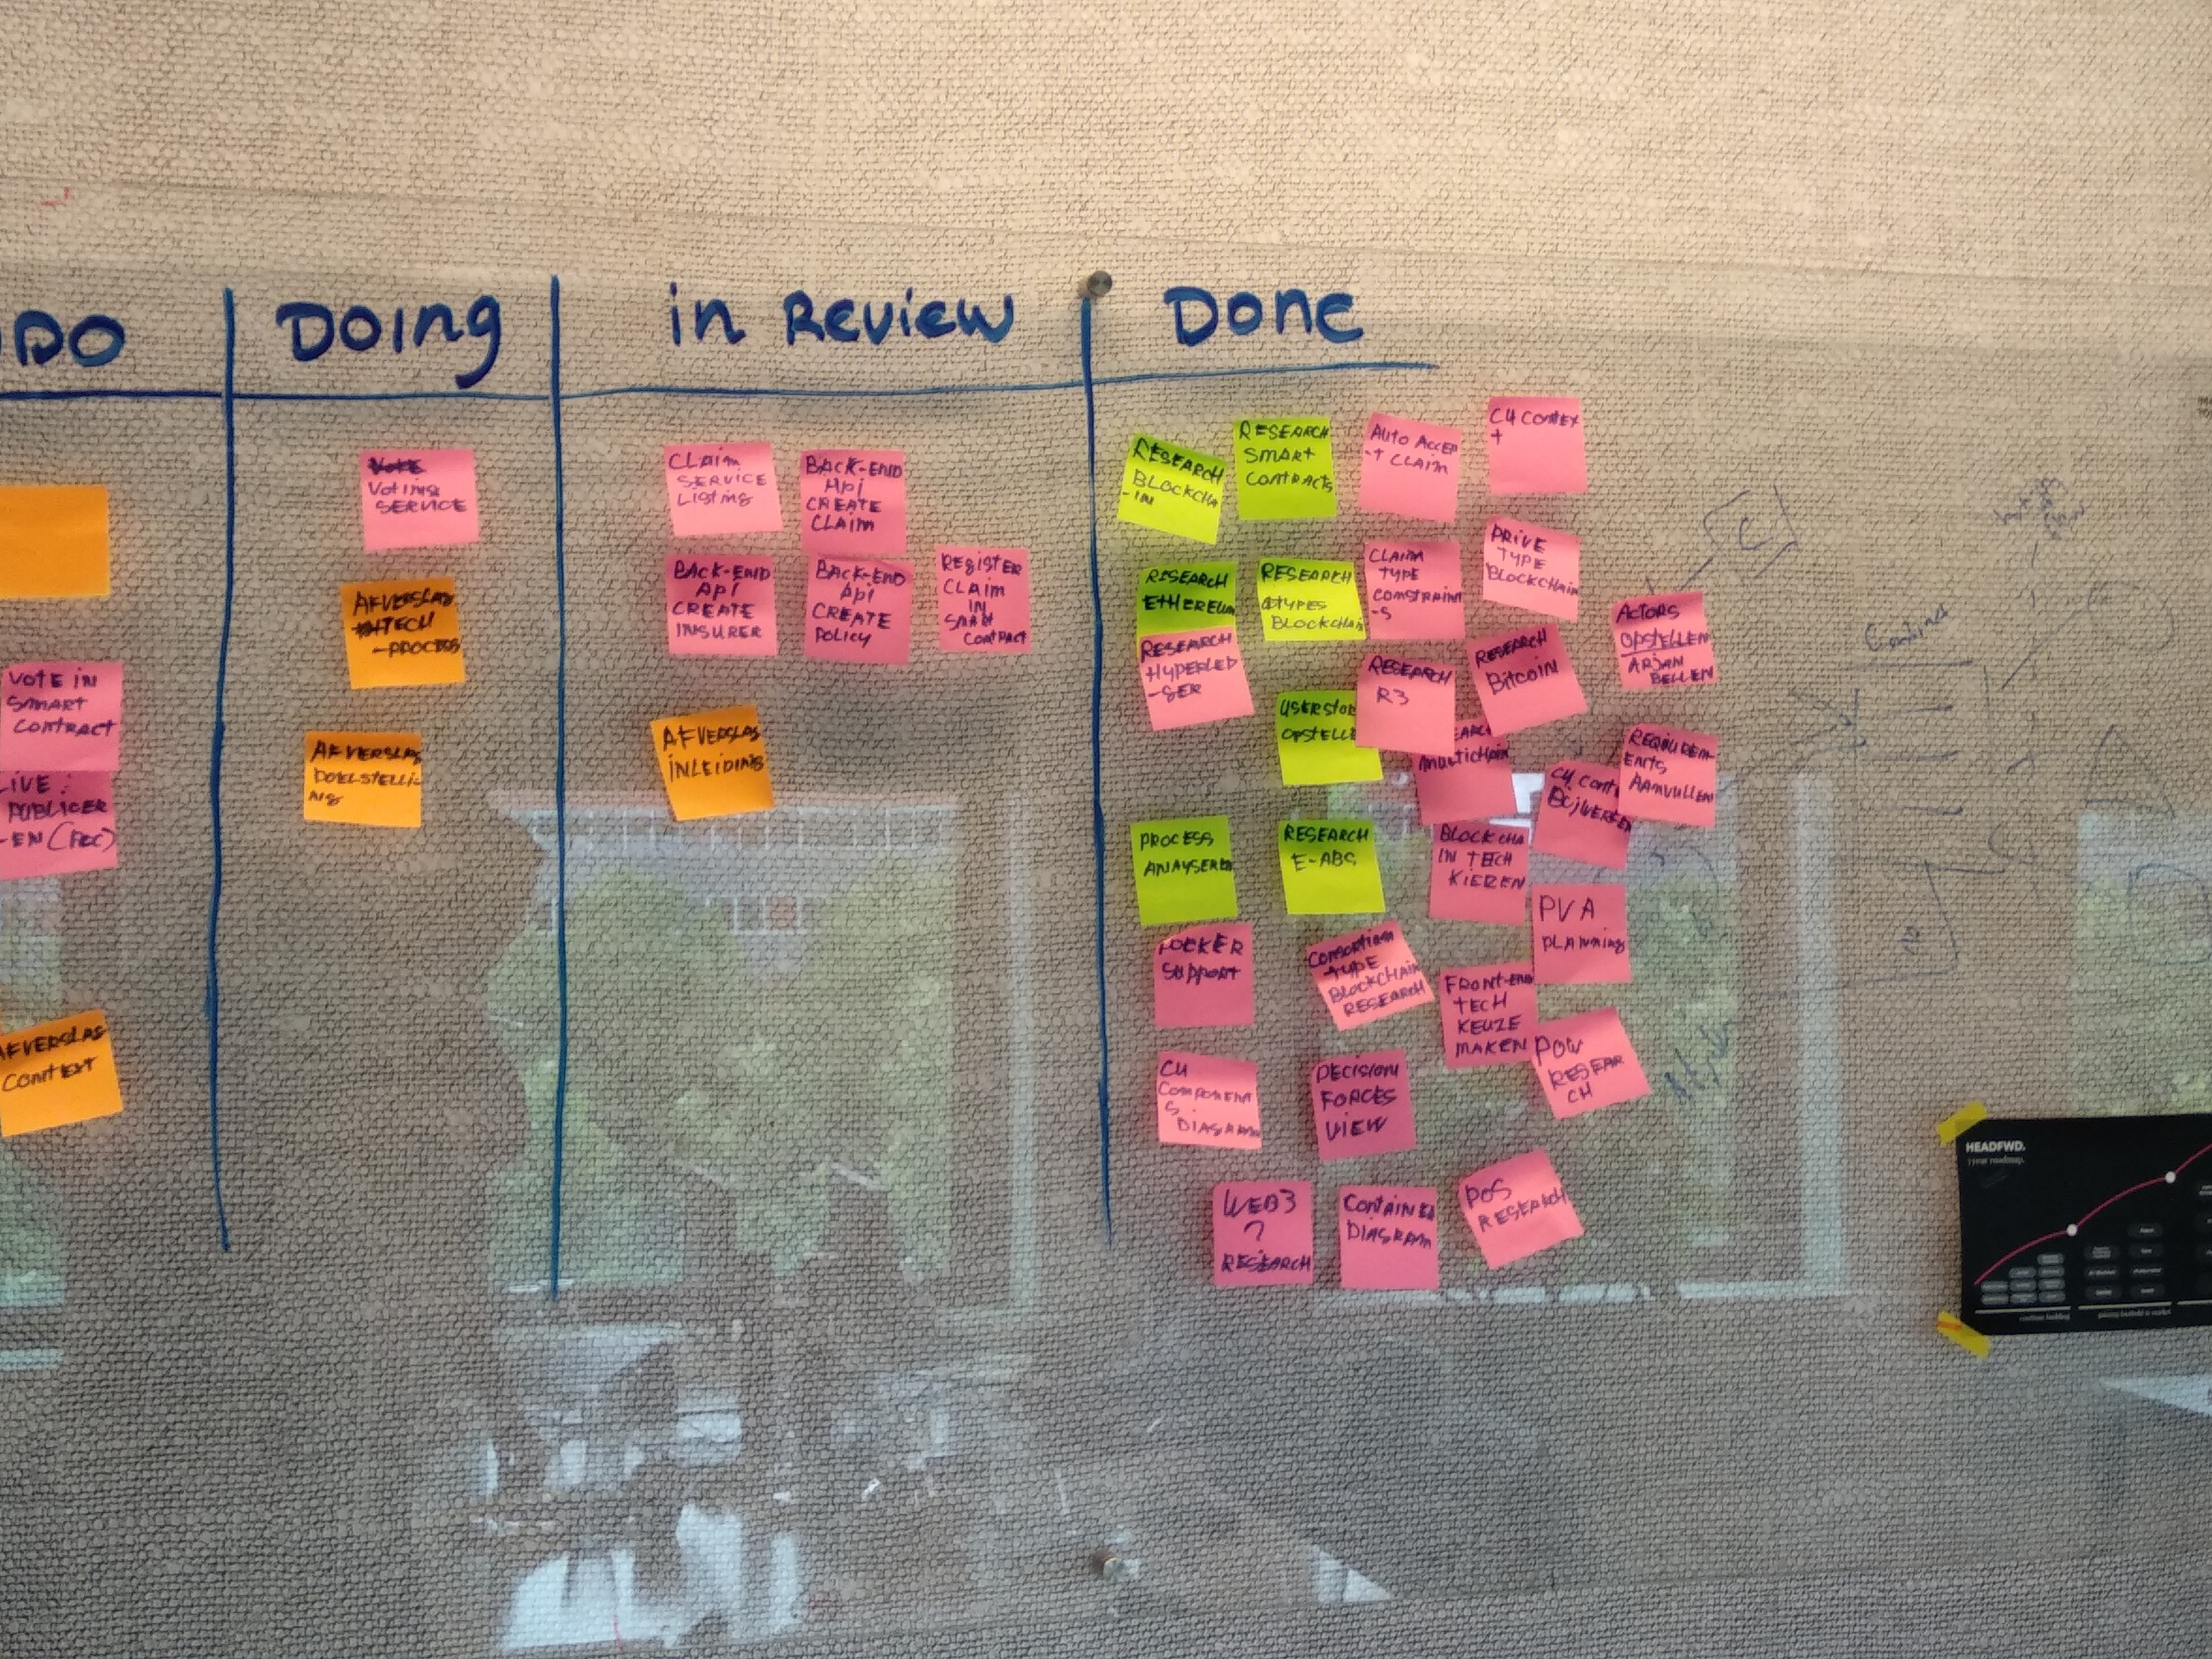
\includegraphics[width=\paperwidth-200pt]{images/kanbanbord}
        \caption{Foto genomen van het Kanban bord op 11-06-2018}
        \label{fig:kanbanbord}
    \end{center}
\end{figure}
\newpage

\section{Technieken}
Er zijn meerdere technieken gebruikt tijdens het project, waarvan een aantal die bekend zijn vanuit de studie. Om te beginnen is er een work breakdown structure gebruikt om werk op te splitsen en vervolgens op te schrijven op post-its op het kanban bord. Om te achterhalen wat de requirements, user stories en het minimum viable product zijn, is er analyse uitgevoerd en verbaal overleg uitgevoerd met de opdrachtgever en de product owner. Deze analyse is vastgelegd in een requirements document en specificeert op een gestructureerde en gestandaardiseerde manier door UML en C4 diagrammen te maken. Deze opgestelde eisen zijn gemaakt gedurende het software- ontwikkeltraject en vervolgens evalueert op basis van gebruikersbehoeften per user story deze door te nemen met de klant. (SD-1)\par
Voor het vermelden van de gebruikte bronnen is de APA richtlijnen \cite{icaControl} gebruikt en tevens verplicht vanuit de HAN. Voor het indelen van de te maken producten en requirements is de MoSCoW-methode toegepast. Er wordt tijdens de ontwikkeling van het proof of concept gebruik gemaakt van GIT, versiebeheer systeem. Waarbij de GitFlow best practice is gebruikt om met iedere nieuwe feature een nieuwe git branch te maken en deze te mergen met een pull-request.\par
Verder is op basis van ontwerp meerdere werkende en betekenisvolle data-intensieve en gedistribueerde software systemen gerealiseerd. Zo is bij de ontwikkeling van het Smart Contract  rekening gehouden met hergebruik, het verminderen van complexiteit en onderhoudbaarheid. Deze code bevat ook de core business rules en is daarom ge-unit test.\par
Er is geen gebruik gemaakt van continuous integration of deployment gezien de tijdsdruk en het feit dat het een prototype is dat na dit afstudeerproject niet verder gebruikt zou worden.\par
Tijdens het onderzoek zijn er prototyping en experimenten uitgevoerd naast literatuuronderzoek. Zo is voor de Blockchain technologie kleinschalig, systematisch en methodisch onderzoek uitgevoerd. De bevindingen en conclusies hieruit hebben geholpen om bepaalde besluiten in het project te onderbouwen.\par
Er is geen digitaal Kanban bord gebruikt zoals Trello of Jira, omdat het fysieke bord voldoende is geweest. Dit is mede mogelijk omdat ik iedere dag op kantoor ben en niemand anders op afstand hier naar hoeft te kijken.
\newpage

\subsection{C4 framework}
Voor het modelleren van de architectuur is er gekozen voor de Simon Brown’s C4 Framework. Deze techniek is mij geleerd tijdens het Advanced Software Development semester. De reden hiervoor was dat door de gekozen agile projectaanpak, software design niet met een heavy upfront design wordt uitgevoerd. Met een agile aanpak wordt bijvoorbeeld UML vooral gebruikt om informele aantekening te maken die bestaan uit vierkanten en lijnen om een verbaal verhaal duidelijk te krijgen. Het probleem hiermee alleen is dat dit niet heel inzichtelijk is of het waard is om in een document mee te nemen.\par
Door het gebruik van C4 framework heb ik een formele manier van communicatie waarmee ik aan de verschillende stakeholders de software architectuur kan uitleggen. Hiermee kan ik agile ontwikkelen en tegelijkertijd de competenties SD-2 en SD-3 vanuit school aantonen en de architectuur duidelijk krijgen. Dit doet C4 door 4 verschillende diagrammen te ontwikkelen met variërende niveaus van abstractie.\par
Deze argumentatie is hetgeen wat mij is geleerd tijdens de SWA lessen en is terug te vinden in slide 11 van de Software Architecture Course: Simon Brown’s C4 Framework \cite{swa11}.